\documentclass[../Article_Design_of_Experiment.tex]{subfiles}
\graphicspath{{\subfix{../Figures/}}}
\begin{document}
	
	\subsubsection{Bayesian Estimation}
	
	After selecting a process model and estimating its parameters based on initial experiments, additional experiments may be planned to further refine the estimates of the model coefficients. An optimal experimental design enables parameters to be estimated without bias and with minimum variance. A model-based approach to experimental design allows for the consideration of system complexity and constraints, such as practical infeasibility due to safety concerns.
	
	Building on the work of \citet{Walter2010} and \citet{Himmelblau1970}, the Bayes' Theorem can be employed to define a general cost function:
	
	{\footnotesize
		\begin{equation}
			\max p\left(\theta \mid Y, \Xi \right) = \frac{p\left(Y \mid \theta, \Xi\right) p\left(\theta\right)}{\int p\left(Y \mid \theta, \Xi\right) p\left(\theta\right) d\theta} \propto p\left(Y \mid \theta, \Xi\right) p\left(\theta\right)
		\end{equation}
	}
	
	The aim of experimental design is to maximize the posterior probability of estimating $\theta$ ($p\left(\theta \mid Y, \Xi \right)$) given the prior distribution of $\theta$ ($p(\theta)$) obtained from previous experiments, and the likelihood of obtaining observations $Y~\left(p\left(Y \mid \theta, \Xi\right)\right)$ given $\theta$ and experimental conditions $\Xi$. The new observations $Y$, under a set of experimental conditions $\Xi$, are assumed to be normally distributed around the model output $y$, with measurement error covariance $\Sigma_Y$. Similarly, $\theta$ is assumed to be normally distributed around the true parameter values $\hat{\theta}$, with covariance matrix $\Sigma_\theta$ estimated from previous experiments. These probabilities are:
	
	{\footnotesize
		\begin{align} 
			p\left(Y \mid \theta, \Xi \right) &= \frac{|\Sigma_Y|^{-1/2}}{\left(2\pi\right)^{n_Y/2}} \exp\left( -\frac{1}{2} \left(Y - y\right)^\top \Sigma_Y^{-1} \left(Y - y\right) \right) \\
			p\left(\theta\right) &= \frac{|\Sigma_\theta|^{-1/2}}{\left(2\pi\right)^{n_\theta/2}} \exp\left( -\frac{1}{2} \left(\theta - \hat{\theta}\right)^\top \Sigma_\theta^{-1} \left(\theta - \hat{\theta}\right) \right)
		\end{align}
	}
	
	where $n_Y$ is the number of observations and $n_\theta$ is the number of parameters to be estimated. By substituting these expressions into the cost function:
	
	{\footnotesize 
		\begin{equation} 
			\ln p\left(\theta \mid Y, \Xi \right) \propto -\frac{1}{2} \left[ \left(Y - y\right)^\top \Sigma_Y^{-1} \left(Y - y\right) + \left(\theta - \hat{\theta}\right)^\top \Sigma_\theta^{-1} \left(\theta - \hat{\theta}\right) \right] 
		\end{equation} }
	
	By linearizing the model output around $\hat{\theta}$, the model output becomes: $y = y(\hat{\theta}) + J \Delta_\theta$, where $J = \frac{\partial y(\hat{\theta})}{\partial \theta}$ is the Jacobian matrix evaluated at $\hat{\theta}$, and $\Delta_\theta = \theta - \hat{\theta}$. To simplify the equation, the residual term $\Delta_y = Y - y(\hat{\theta})$ is introduced. Substituting these into the expression for $\ln p\left(\theta \mid Y, \Xi \right)$:
	
	{\footnotesize 
		\begin{flalign*} 
			\ln p\left(\theta \mid Y, \Xi \right) &\propto -\frac{1}{2} \left[ \left(\Delta_y - J \Delta_\theta \right)^\top \Sigma_Y^{-1} \left(\Delta_y - J \Delta_\theta \right) + \Delta_\theta^\top \Sigma_\theta^{-1} \Delta_\theta \right] && \\
			&= -\frac{1}{2} \left[ \Delta_y^\top \Sigma_Y^{-1} \Delta_y - 2 \Delta_y^\top \Sigma_Y^{-1} J \Delta_\theta + \Delta_\theta^\top \left( J^\top \Sigma_Y^{-1} J + \Sigma_\theta^{-1} \right) \Delta_\theta \right] &&
		\end{flalign*} }
	
	This equation can be reformulated by expanding the quadratic terms:
	
	{\footnotesize
		\begin{flalign*}
			\ln p\left(Y \mid \theta, \Xi \right) &\propto -\frac{1}{2} \left( \underbrace{r^\top \Sigma_Y^{-1} r}_{C} - 2 \underbrace{ J^\top \Sigma_Y^{-1} \Delta_y }_{B} \Delta_\theta + \Delta_\theta^\top \underbrace{\left( J^\top \Sigma_Y^{-1} J + \Sigma_\theta^{-1} \right)}_{A} \Delta_\theta \right) && \\
			&=-\frac{1}{2} \left( \Delta_\theta^\top A \Delta_\theta - 2 B^\top \Delta_\theta + C \right) &&
		\end{flalign*}
	}
	
	By completing the square, we introduce $\theta^* = \hat{\theta} + A^{-1} B$, and the cost function becomes:
	
	{\footnotesize 
		\begin{equation} 
			\ln p\left(\theta \mid Y, \Xi \right) \propto -\frac{1}{2} \left( \left( \theta - \theta^* \right)^\top A \left( \theta - \theta^* \right) + C - B^\top A^{-1} B \right) 
		\end{equation} }
	
	It can be observed that the quadratic term represents the spread of the posterior multivariate distribution around the mean $\theta^*$. The constant term $C - B^\top A^{-1} B$ is independent of $\theta$ and does not affect the shape of the posterior distribution but is still important for normalization. This constant term is absorbed into the normalizing constant of the posterior distribution. It does not affect the estimation of $\theta$ or the shape of the posterior distribution and thus can be neglected when focusing on parameter estimation or experimental design. Therefore, the posterior distribution of $\theta$ given $Y$ and $\Xi$ is:
	
	{\footnotesize \begin{equation} p\left(\theta \mid Y, \Xi \right) \propto \exp \left( -\frac{1}{2} \left( \theta - \theta^* \right)^\top A \left( \theta - \theta^* \right) \right) \end{equation} }
	
	This is the expression of a multivariate normal distribution with mean $\theta^*$ and covariance matrix $A^{-1}$:
	
	{\footnotesize \begin{equation} p\left(\theta \mid Y, \Xi \right) = \mathcal{N}\left( \theta^*, A^{-1} \right) \end{equation} }
	
	As the goal of optimal experimental design is to improve the precision of parameters, the main focus is on the matrix $A$, which consists of two terms. The first corresponds to the information gained from new observations based on the model and measurement error ($J^\top \Sigma_Y^{-1} J$), while the second is the prior information ($\Sigma_\theta^{-1}$).
	
	\subsubsection{Fisher Information}
	
	The Fisher Information $\mathcal{F}$ measures the amount of information that an observable random variable carries about an unknown parameter of the distribution that models the random variable. It is related to the negative expected value of the second derivative of the log-likelihood function with respect to the parameter, providing a measure of how "sensitive" the likelihood is to changes in the parameter value.
	
	{\footnotesize \begin{equation} \mathcal{F}(\theta, \Xi) = -\mathop{\mathbb{E}}_{Y \mid \theta, \Xi} \left[ \frac{\partial^2 \ln p \left( Y \mid \theta, \Xi \right)}{\partial \theta \partial \theta^\top} \right] \end{equation} }
	
	Under regularity conditions, the Fisher Information can also be expressed as:
	
	{\footnotesize \begin{equation} \mathcal{F}(\theta, \Xi) = \mathop{\mathbb{E}}_{Y \mid \theta, \Xi} \left[ \left( \frac{\partial \ln p\left( Y \mid \theta, \Xi \right)}{\partial \theta} \right) \left( \frac{\partial \ln p\left( Y \mid \theta, \Xi \right)}{\partial \theta} \right)^\top \right] \end{equation} }
	
	By inserting the expression for $p\left( Y \mid \theta, \Xi \right)$ and performing similar manipulations as in the previous section, the Fisher Information becomes:
	
	{\footnotesize \begin{equation} \mathcal{F}(\theta, \Xi) = J^\top \Sigma_Y^{-1} J \end{equation} }
	
	Since the likelihood is Gaussian and linearized, the second derivative of the log-likelihood with respect to $\theta$ simplifies to $J^\top \Sigma_Y^{-1} J$, and its negative expected value yields the same expression because the expectation of the Hessian is constant in this linear approximation.

	The Cramér-Rao inequality provides that the covariance of any unbiased estimator $\hat{\theta}$ satisfies:
	
	{\footnotesize \begin{equation} \operatorname{Cov}(\hat{\theta}) \geq \mathcal{F}^{-1}(\theta) \end{equation} }
	
	The precision with which a parameter $\theta$ can be estimated is limited by the Fisher Information of the likelihood function. Based on the Cramér-Rao inequality, the Fisher Information matrix can be used to calculate the covariance matrices associated with maximum-likelihood estimates.
	
	\subsubsection{Optimal experimental design}
	
	The optimal design of experiments is a statistical concept that refers to the process of planning an experiment that allows parameters to be estimated without bias and with minimum variance. Optimal design ensures that the experiment can provide the most informative data possible. This often involves balancing the study of main effects and interactions between factors. Moreover, by efficiently planning experiments, optimal design aims to reduce the overall resources required, such as time, materials, and manpower.
	
	The methodology for collecting data to estimate the parameters of a specific model is influenced by a series of qualitative decisions made throughout the experimental and modeling process, such as model structure, sensor locations, or equipment choices. Once these choices have been made, the experimenter still has some freedom to specify the quantitative experimental conditions (such as temperature, pressure, sampling times, etc.). Experiment design aims to determine experimental conditions adapted to the final purpose of the modeling.
	
	Consider that each scalar observation in a study can be expressed as $y(\xi_i)$, where the $n_\xi$-dimensional vector $\xi_i$ represents the specific experimental conditions (such as sampling time, operating conditions, etc.) under which the $i$-th observation is gathered. When collecting $n_t$ such observations, the assembly of these $\xi_i$ vectors forms the matrix $\Xi = (\xi_1, \xi_2, \dots, \xi_{n_t})$, which combines all the experimental conditions that need optimization. To align the design of the experiment with practical realities, it's important to take into account various constraints, such as the total duration of the experiments, the maximum temperature of the inlet stream, or the minimum interval between sampling events. The set of all possible combinations for $\Xi$ that adhere to these constraints is denoted as $\bar{\Xi}$.
	
	The formulation of a cost function $j$ allows for the framing of optimal experiment design as a problem of constrained optimization. In this context, the optimal experiment, denoted as $\Xi^*$, is:
	
	{\footnotesize \begin{equation} \Xi^* = \arg~\underset{\Xi \in \bar{\Xi}}{\text{opt}}~j\left(\Xi\right) \end{equation} }
	
	The cost function should describe the amount of information obtained from an experiment. For that purpose, it can be assumed that a function $\kappa$ can be related to the covariance matrix $A^{-1}$ obtained at arbitrary operating conditions:
	
	{\footnotesize \begin{equation} j(\Xi) = \kappa\left[ A^{-1}(\theta, \Xi) \right] \end{equation} }
	
	Recall that in the Bayesian estimation framework, the posterior covariance matrix of the parameter estimates is given by $\Sigma = A^{-1} = \left(J^\top \Sigma_Y^{-1} J + \Sigma_\theta^{-1}\right)^{-1} $. $J$ is the Jacobian matrix of the model outputs with respect to the parameters, $\Sigma_Y$ is the covariance matrix of the measurement errors, and $\Sigma_\theta$ is the prior covariance matrix of the parameters.
	
	\begin{figure}[!h]
		\centering
		\resizebox{1\columnwidth}{!}{%
			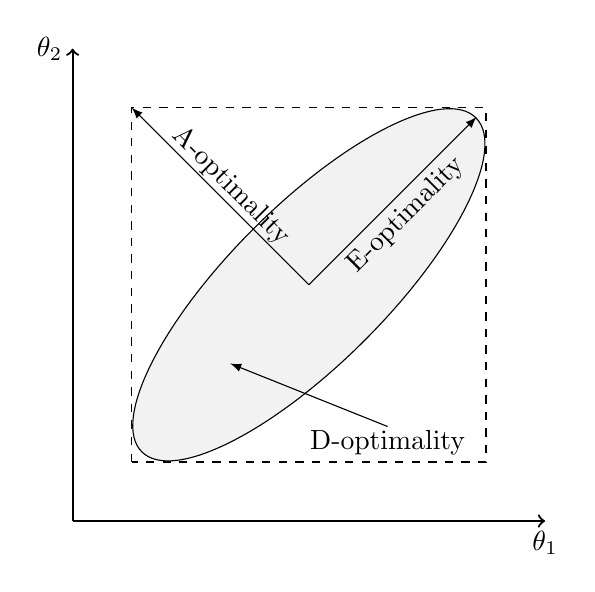
\begin{tikzpicture}
				% Ellipse parameters
				\def\ellipsecenter{(3,3)}
				\def\ellipseA{(0.75,5.25)} % End point for A-optimality arrow
				\def\ellipseB{(5.13,5.13)} % End point for E-optimality arrow
				\def\ellipseC{(4,1.2)}      % End point for D-optimality arrow
				
				% Draw the rotated ellipse
				\draw[fill=gray!10, draw=black, rotate around={45:\ellipsecenter}] \ellipsecenter ellipse (3cm and 1cm);
				
				% Draw the dashed rectangle
				\draw[dashed] (0.75,0.75) rectangle (5.25,5.25);
				
				% Draw the arrows and label them with adjustable positions
				\draw [-latex] \ellipsecenter -- \ellipseA node[yshift=-4cm, xshift=2.5cm,rotate around={-45:\ellipsecenter}] {A-optimality};
				\draw [-latex] \ellipsecenter -- \ellipseB node[yshift=0cm, xshift=-3.9cm,rotate around={45:\ellipsecenter}] {E-optimality};
				\draw [-latex] \ellipseC -- (2,2) node[yshift=-1cm, xshift=2cm] {D-optimality};
				
				% Draw axes
				\draw[thick,->] (0,0) -- (6,0) node[below] {$\theta_1$};
				\draw[thick,->] (0,0) -- (0,6) node[left] {$\theta_2$};
			\end{tikzpicture}
		}%
		\caption{Graphical representation of score functions}
		\label{fig:score_fun}
	\end{figure}
	
	A general class of design of experiments (DOE) optimality criteria is given by Equation \ref{EQ:DOE_general}. Some of the DOE criterion have graphical interpretation as shown in Figure \ref{fig:score_fun}.
	
	{\footnotesize 
		\begin{align} \label{EQ:DOE_general}
			\kappa_k\left( A^{-1}(\theta) \right) &= \left[ \frac{1}{n_\theta} \operatorname{trace}\left( Q A^{-1}(\theta, \Xi) Q^\top \right)^k \right]^{1/k} & \text{if} \det A^{-1} \neq 0, \nonumber \\ 
			\kappa_k\left( A^{-1}(\theta) \right) &= \infty & \text{if} \det A^{-1} = 0
		\end{align} }
	
	where $Q$ is a weighting matrix. The special case $k=1$ corresponds to the L-optimality cost function:
	
	{\footnotesize \begin{equation} j_L(\Xi) = \operatorname{trace} \left( Q A^{-1}(\theta, \Xi) Q^\top \right) \end{equation} }
	
	Choosing $Q = \mathbf{I}_{n\theta}$ corresponds to the A-optimality cost function. An A-optimal experiment minimizes the sum of the variances of the parameter estimates (i.e., the trace of the covariance matrix). When $Q$ is diagonal with $[Q]_{ii} = 1/\theta_i$, this corresponds to weighting the parameters inversely by their magnitude, which is associated with relative precision.
	
	Selecting $Q$ as a row vector results in C-optimality, which focuses on linear combinations of parameters. Setting $Q = \mathbf{I}_{n\theta}$ and $k = \infty$ leads to E-optimality, where the design maximizes the smallest eigenvalue of the covariance matrix $A^{-1}(\theta, \Xi)$, thereby minimizing the length of the largest axis of the asymptotic confidence ellipsoids.
	
	The most commonly used criterion is the D-optimality, which involves $k = 0$ and $Q = \mathbf{I}_{n\theta}$, requiring the minimization of $\det A^{-1}(\theta, \Xi)$, or equivalently, maximization of:
	
	{\footnotesize \begin{equation} j_D(\Xi) = \det A(\theta, \Xi) \end{equation} }
	
	Since $\det A(\theta, \Xi) = 1 / \det A^{-1}(\theta, \Xi)$, maximizing $\det A$ is equivalent to minimizing $\det A^{-1}$.
	
	The D-optimality (D-OED) criterion originates from the geometric interpretation of the determinant. A two-dimensional matrix with real number entries can represent two linear maps: one mapping the standard basis vectors to the rows and the other to the columns. In both cases, the images of the basis vectors form a parallelogram that represents the image of the unit square under the mapping. The absolute value of the determinant is the area of this parallelogram, reflecting the scale factor by which the matrix transforms areas. The signed value of the determinant indicates the area of the parallelogram, which is negative when the angle from the first to the second defining vector is clockwise. In the multi-dimensional case, the matrix maps the n-cube to an n-dimensional parallelotope. The determinant provides the signed n-dimensional volume of this parallelotope, describing the volume scaling factor of the linear transformation produced by the matrix. Based on this geometrical interpretation, a D-optimal experiment minimizes the volume of the asymptotic confidence ellipsoids for the parameters.
	
	\subsubsection{Problem formulation}
	
	Details on the process model can be found in \citet{Sliczniuk2024}. The model's empirical correlations are derived based on laboratory experiments conducted under various but constant operating conditions: $30^\circ\text{C} - 40^\circ\text{C}$, $100 - 200$ bar, and $3.33 \cdot 10^{-5} - 6.67 \cdot 10^{-5}$ kg/s. This study employs the process model obtained previously to design a set of supplementary experiments with dynamically changing conditions to improve the precision of the correlation for $D_i$. The analyzed correlations consist of three independent variables: mass flow rate, pressure and inlet temperature. 
	
	In this work, the decision variables are the inlet temperature ($T^{\text{in}}$) and mass flow rate ($F$), while the pressure is assumed to remain constant during a batch. The optimal design of experiment problem is solved for multiple values of pressure: 100, 125, 150, 175, and 200 bar. The initial state is considered isothermal, so $T^0(z) = T^{\text{in}}(t=0)$.
	
	The decision variables are adjusted every 10 minutes and are kept constant within each interval (piecewise constant controls). These controls have lower and upper bounds that match the validated range of the process model detailed by \citet{Sliczniuk2024}. The sampling time is assumed to be 5 minutes, and the total extraction time is 600 minutes. The standard deviation $\sigma^2$ was estimated to be 0.03.
	
	In a real system, the mass flow rate and inlet temperature cannot be changed instantaneously to any arbitrary value, as they depend on the dynamics of the pump and heat exchanger, respectively. To prevent bang-bang type of control, a penalty term is introduced. Inspired by control problems, such as the Linear Quadratic Regulator, a quadratic penalty term is added to the cost function. This penalty increases the cost function value when there are rapid changes in the decision variables. The matrix $\bar{R}$ represents the control cost matrix, with its entries chosen so that the control costs are one order of magnitude lower than $-\ln j_D$. The problem formulation is given by Equation \ref{EQ:Formulation_2}.
	
	{\footnotesize 
		\begin{equation} 
			\begin{aligned} \Xi^* &= \arg \min_{ T^{\text{in}}(t), F(t) } \int_{t_0}^{t_f} \left[ - \ln j_D(\Xi, \dot{x}) + \frac{du(t)^\top}{dt}~\bar{R}~\frac{du(t)}{dt} \right] dt \\ 
				\text{subject to} \quad & \dot{x} = G(x, t, \theta; \Xi), \\ 
				& t_0 = 0 \text{min} \\ 
				& t_f = 600 \text{min} \\ 
				& T^{0} = T^{\text{in}}(t=0), \\ 
				& P(t) \in \left\{100, 125, 150, 175, 200\right\} \text{bar}, \\ 
				& 30^\circ\text{C} \leq T^{\text{in}}(t) \leq 40^\circ\text{C}, \\ 
				& 3.33 \cdot 10^{-5} \leq F(t) \leq 6.67 \cdot 10^{-5} \\
				& \bar{R} = \begin{bmatrix} 0.1 & 0 \\ 0 & 0.01 \end{bmatrix} \\ 
				& \frac{du(t)}{dt} = \begin{bmatrix} \dfrac{dF(t)}{dt} \\ \dfrac{dT^{\text{in}}(t)}{dt} \end{bmatrix}
				\end{aligned} 
				\label{EQ:Formulation_2} 
			\end{equation} }
	
\end{document}













































